\section{Introduction}
\label{sec:intro}
%
Phase Change Memory (PCM) is a recently developed non-volatile memory
technology, constructed from chalcogenide glass material, that stores
data by switching between amorphous (\emph{binary 0}) and crystalline 
(\emph{binary 1}) states. Broadly speaking, it is expected to provide an attractive
combination of the best features of conventional disks (persistence,
capacity) and of DRAM (access speed). For instance, it is
about 2 to 4 times denser than DRAM, while providing a DRAM-comparable
read latency.  On the other hand, it consumes much less energy
than magnetic hard disks while providing substantively smaller write latency. Due to this suite of  desirable features, PCM technology is
expected to play a prominent role in the next generation of computing
systems, either augmenting or replacing current components in the memory
hierarchy~\cite{qureshi,zhou,lee}.

A limitation of PCM, however, is that there is a significant difference
between the read and write behaviors in terms of energy, latency and
bandwidth. A PCM write, for example, consumes 6 times more energy than
a read. Further, PCM has limited write endurance since a memory cell
becomes unusable after the number of writes to the cell exceeds a threshold
determined by the underlying glass material. Consequently, several database
researchers have, in recent times, focused their attention on devising
new implementations of the core database operators that are adapted to
the idiosyncrasies of the PCM environment (e.g.~\cite{chen,viglas}). 

\subsection*{Architectural Model}
The prior database work has primarily focused on computing
architectures wherein either (a) PCM completely replaces the
DRAM memory~\cite{chen}; or (b) PCM and DRAM co-exist side-by-side
and are independently controlled by the software~\cite{viglas}. We
hereafter refer to these options as {\bf \modelPcmRam{}} and
{\bf \modelExplicit{}}, respectively.

However, a third option that is gaining favor in the architecture
community, and also mooted in \cite{chen} from the database
perspective, is where the PCM is augmented with a small hardware-managed
DRAM buffer~\cite{qureshi}. In this model, which we refer to as {\bf
\model{}}, the address space of the application maps to PCM, and the DRAM
buffer can simply be visualized as yet another level of the existing
cache hierarchy.  For ease of comparison, these various configurations
are pictorially shown in Figure~\ref{fig:pcm_models}.

\begin{figure}[t]
	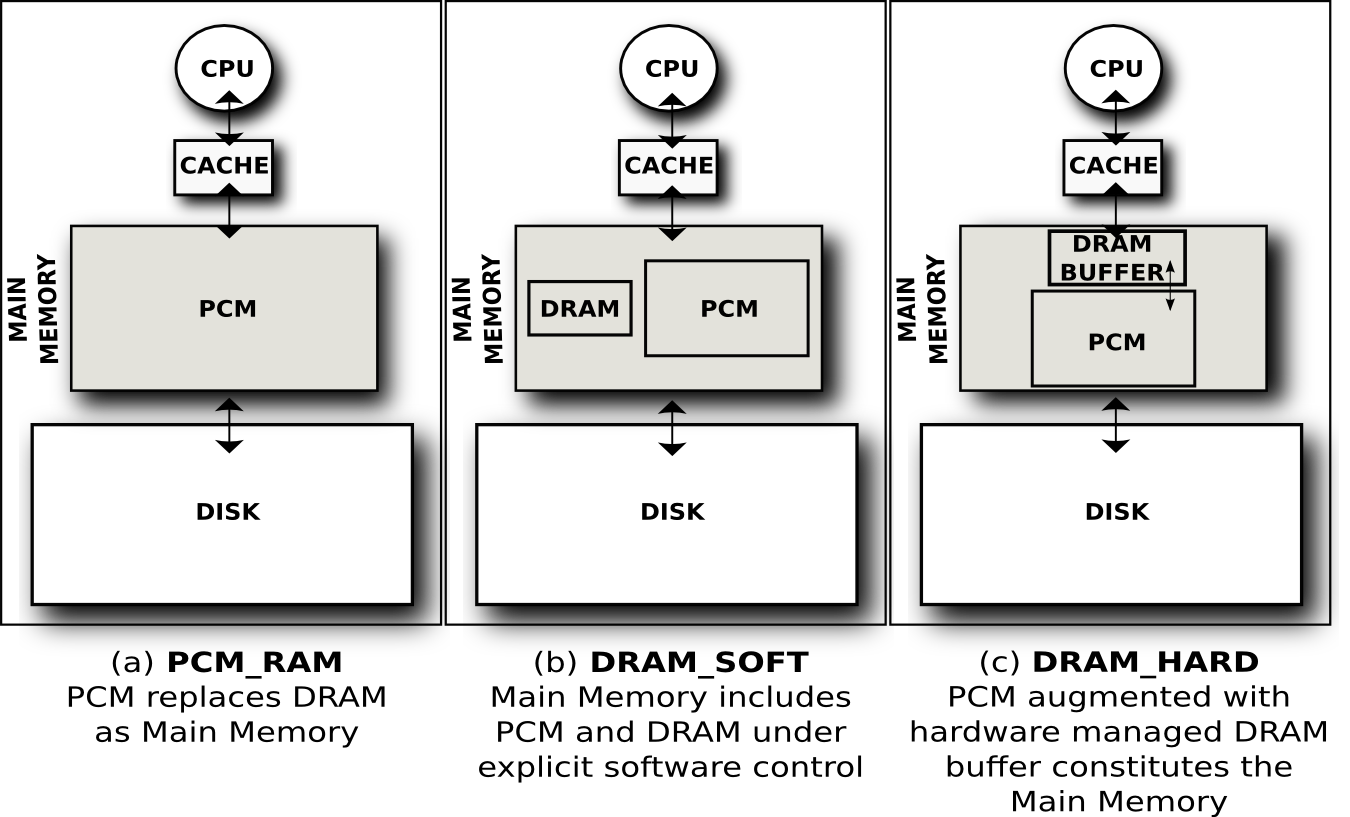
\includegraphics[height=80mm]{./fig/PCM_Models.png}\centering
	\caption{PCM-based Architectural Options \cite{chen}}
	\label{fig:pcm_models}
\end{figure}

There are several practical advantages of the \model{} configuration:
First, the write latency drawback of \modelPcmRam{} can be largely
concealed by the intermediate DRAM buffer~\cite{qureshi}. Second,
existing applications can be used \textit{as is} but still manage to take
advantage of both the DRAM and the PCM. This is in stark contrast to the
\modelExplicit{} model which requires incorporating additional machinery,
either in the program or in the OS, to distinguish between data mapped
to DRAM and to PCM -- for example, by having separate address space
mappings for the different memories.

\subsection*{Our Work}
In this paper, we propose minimalist reworkings, that are tuned to
the \model{} model,  of current implementations of database operators.
In particular, we focus on the ``workhorse'' operators:
\textit{sort}, \textit{hash join} and \textit{group-by}.
The proposed modifications are not only easy to implement but are attractive from the performance perspective also, simultaneously reducing
\emph{both} PCM writes and query response times.
The new implementations are evaluated on Multi2sim
\cite{multi2sim}, a state-of-the-art architectural simulator, after
incorporating major extensions to support modelling of the \model{}
configuration.  Their performance is evaluated on \emph{complete}
TPC-H benchmark queries. This is a noteworthy point since earlier studies
of PCM databases had only considered operator performance in isolation.
But, it is possible that optimizing a specific operator may turn out to be detrimental
to downstream operators that follow it in the query execution plan. For
instance, the proposal in \cite{chen} to keep leaf nodes unsorted in B$^+$
indexes -- while this saves on writes, it is detrimental to the running
times of \emph{subsequent} operators that leverage index ordering -- for instance, \emph{join filters}.
Finally, we include the metric of \emph{wear distribution}
in our evaluation to ensure that the reduction in writes is not achieved
at the cost of skew in wear-out of PCM cells.

Our simulation results indicate that the customized implementations
collectively offer substantive benefits with regard to PCM writes --
the number is typically brought down \emph{by a factor of two to three}.
Concurrently, the query response times are also brought down by about
\emph{20--30 percent}. As a sample case in point, for TPC-H Query 19,
savings of 64\% in PCM writes are achieved with a concomitant 32\%
reduction in CPU cycles. 

Fully leveraging the new implementations requires integration with
the query optimizer, an issue that has been largely overlooked in
the prior literature. We take a first step here by providing simple
but effective statistical \emph{estimators} for the number of writes
incurred by the new operators,
and incorporating these estimators in the query optimizer's cost model.
Sample results demonstrating that the resultant plan choices provide
substantively improved performance are provided in our experimental study.

Overall, the above outcomes augur well for the impending migration
of database engines to PCM-based computing platforms.

\subsection*{Organization}
The remainder of this paper is organized as follows: We define the
problem framework in Section~\ref{sec:framework}. The design of the new
PCM-conscious database operators, and an analysis of their PCM writes,
are presented in Sections~\ref{sort}, \ref{hj} and \ref{gby}.
Our experimental framework and the simulation results are reported in
Sections~\ref{sec:exp} and \ref{sec:results}, respectively. This is followed by a
discussion in Section~\ref{integration} on integration with the query optimizer. 
The related literature is reviewed in Section~\ref{relWork}. Finally,
Section~\ref{conclusion} summarizes our conclusions and outlines future
research avenues.
